\documentclass[tikz,border=9pt]{standalone}
\usepackage{amsmath}
\usepackage{array}
\usetikzlibrary{arrows.meta,calc,positioning}
\definecolor{starkblue}{HTML}{0072B2}
\definecolor{starkgreen}{HTML}{009E73}
\definecolor{starkgold}{HTML}{E69F00}
\definecolor{starkpurple}{HTML}{CC79A7}
\definecolor{starkred}{HTML}{D55E00}
\begin{document}
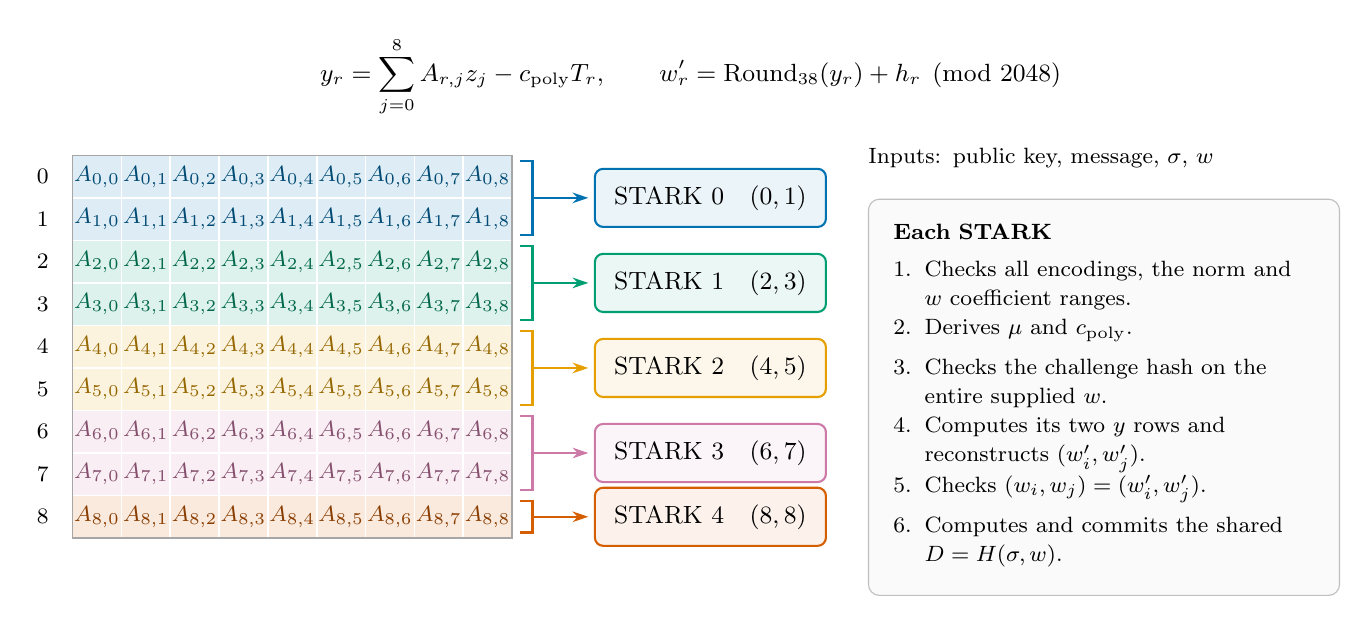
\begin{tikzpicture}[font=\fontsize{9}{11}\selectfont,
 arrow/.style={-{Stealth[length=2mm,width=1.35mm]},line width=.75pt},
 proof/.style={rounded corners=3pt,draw,line width=.75pt,
   inner xsep=7pt,inner ysep=6pt,minimum width=2.3cm,minimum height=.65cm,align=center},
 note/.style={font=\fontsize{8.5}{10.5}\selectfont,align=left}]

\node at (8.25,1.0) {$y_r=\displaystyle\sum_{j=0}^{8}A_{r,j}z_j-c_{\mathrm{poly}}T_r,
 \qquad w'_r=\operatorname{Round}_{38}(y_r)+h_r\pmod{2048}$};

\foreach \r in {0,...,8} {
  \ifnum\r<2 \def\rowcolor{starkblue}\else
  \ifnum\r<4 \def\rowcolor{starkgreen}\else
  \ifnum\r<6 \def\rowcolor{starkgold}\else
  \ifnum\r<8 \def\rowcolor{starkpurple}\else
  \def\rowcolor{starkred}\fi\fi\fi\fi
  \pgfmathsetmacro{\yc}{-.54*\r}
  \node[anchor=east,font=\fontsize{8}{10}\selectfont] at (.22,\yc-.27) {\r};
  \foreach \j in {0,...,8} {
    \pgfmathsetmacro{\xc}{.40+.62*\j}
    \path[fill=\rowcolor!13,draw=white,line width=.6pt]
      (\xc,\yc) rectangle ++(.62,-.54);
    \node[font=\fontsize{8}{10}\selectfont,text=\rowcolor!65!black]
      at (\xc+.31,\yc-.27) {$A_{\r,\j}$};
  }
}
\draw[black!35,line width=.5pt] (.40,0) rectangle (5.98,-4.86);

\foreach \p/\ya/\yt/\yb/\ra/\rb/\col in {
 0/-.54/0/-1.08/0/1/starkblue,
 1/-1.62/-1.08/-2.16/2/3/starkgreen,
 2/-2.70/-2.16/-3.24/4/5/starkgold,
 3/-3.78/-3.24/-4.32/6/7/starkpurple,
 4/-4.59/-4.32/-4.86/8/8/starkred} {
  \node[proof,draw=\col,fill=\col!8] (S\p) at (8.5,\ya)
    {STARK \p\quad $(\ra,\rb)$};
  \draw[draw=\col,line width=.8pt]
    (6.08,\yt-.07) -- (6.24,\yt-.07) -- (6.24,\yb+.07) -- (6.08,\yb+.07);
  \draw[arrow,draw=\col,shorten >=2pt] (6.24,\ya) -- (S\p.west);
}

\node[note,text width=5.85cm,anchor=north west,inner sep=0pt] at (10.5,.10)
  {Inputs: public key, message, $\sigma$, $w$};
\node[draw=black!25,fill=black!2,rounded corners=4pt,
  text width=5.35cm,inner sep=9pt,align=left,anchor=north west,
  font=\fontsize{8.5}{10.5}\selectfont] at (10.5,-.55) {%
  \textbf{Each STARK}\par\vspace{5pt}
  \begin{minipage}{\linewidth}
  \setlength{\parindent}{0pt}
  \begin{tabular}{@{}r@{\hspace{.55em}}>{\raggedright\arraybackslash}p{4.85cm}@{}}
  1. & Checks all encodings, the norm and $w$ coefficient ranges.\\[4pt]
  2. & Derives $\mu$ and $c_{\mathrm{poly}}$.\\[4pt]
  3. & Checks the challenge hash on the entire supplied $w$.\\[4pt]
  4. & Computes its two $y$ rows and reconstructs $(w'_i,w'_j)$.\\[4pt]
  5. & Checks $(w_i,w_j)=(w'_i,w'_j)$.\\[4pt]
  6. & Computes and commits the shared $D=H(\sigma,w)$.
  \end{tabular}
  \end{minipage}};

\end{tikzpicture}
\end{document}
